\documentclass[14pt]{article} % article
\usepackage[utf8]{inputenc}
\usepackage{listingsutf8}
%\usepackage[T2A]{fontenc}
\usepackage[english]{babel}
\usepackage{amssymb,amsmath,amsfonts,amsbsy}
%\usepackage{mathtext}
%\usepackage{indentfirst}
\usepackage{tabularx}
\usepackage{booktabs}
\usepackage{graphicx}
\usepackage[center]{caption}
\captionsetup{justification=raggedright,singlelinecheck=false}
\usepackage{subcaption}
\usepackage{cite}
\usepackage{enumerate}
\usepackage{enumitem}
%%\usepackage[braket]{qcircuit}
\usepackage{marvosym}
\usepackage{multicol}
\usepackage{comment}
\usepackage{authblk}
\usepackage{lipsum}
%\usepackage{hyperref}
\graphicspath{{figs/}}
%\DeclareGraphicsExtensions{.pdf,.png,.jpg}
%\bibliographystyle{utf8gost780u}
%\usepackage{apacite}
%\bibliographystyle{apacite}

% Print line number page wisely 
%\usepackage[pagewise]{lineno}
%\linenumbers

%\renewcommand\linenumberfont{\normalfont\bfseries\normal}
%\renewcommand\linenumberfont{\normal}

\title{\vspace{-2.5cm}\textbf{Exploring the Shared Low-Dimensional Subspace of EEG and EOG Signals in Sleep Stages}}

%\author[1]{Ilia Golub}
\author[]{Ilia Golub}

%\author[1]{Pratit Kandel}

%\author[1]{Prosperity Oguama}
\author[]{Xueqing Li}


%\affil[1]{Gonda Multidisciplinary Brain Research Center, Bar-Ilan University, Ramat Gan, Israel}
\affil[]{Gonda Multidisciplinary Brain Research Center, Bar-Ilan University, Ramat Gan, Israel}
%\affil[4]{Institute of Natural Sciences and Mathematics, Ural Federal University, Ekaterinburg, Russia}
%\affil[5]{Department of Cardiology, Clinical Sciences, Lund University, Lund, Sweden}
%\affil[6]{Arrhythmia Clinic, Skane University Hospital, Lund, Sweden}
%\affil[*]{Correspondence: golub.ilia.ilya@gmail.com}

\setcounter{Maxaffil}{0}
\renewcommand\Affilfont{\itshape\small}
\date{}

\usepackage[onehalfspacing]{setspace}

\usepackage{listings}
\renewcommand{\lstlistingname}{Listing}
\lstset{language=Python,
        numbers=left,
        basicstyle=\small\ttfamily,
        breaklines=true,
        showstringspaces=false,
        stepnumber=1,         
        numbersep=5pt,          
        showspaces=false,       
        showtabs=false,         
        %frame=single,          
        tabsize=4,              
        captionpos=b,           
        breakatwhitespace=false,
        escapeinside={\%*}{*)}, 
        texcl=true
        }

%\usepackage[left=1cm, right=1cm, top=1cm, bottom=1cm]{geometry} % 2.5 1 1 2.5
\usepackage[a4paper, margin=0.5in]{geometry}


\usepackage[
    colorlinks=true,
    linkcolor=blue,
    filecolor=magenta,      
    urlcolor=cyan,
    pdftitle={CW-2},
    pdfauthor={Golub I},
    bookmarks=true,
    linktoc=all,
	final]{hyperref}

\usepackage[nottoc]{tocbibind}

\makeatletter
\renewcommand{\@biblabel}[1]{#1.}
\makeatother

\sloppy

\righthyphenmin=2

\renewcommand{\theenumi}{\arabic{enumi}.}
\renewcommand{\labelenumi}{\arabic{enumi}.} 
\renewcommand{\theenumii}{\arabic{enumii}.} 
\renewcommand{\labelenumii}{\arabic{enumi}.\arabic{enumii}.}
\renewcommand{\theenumiii}{\arabic{enumiii}.} 
\renewcommand{\labelenumiii}{\arabic{enumi}.\arabic{enumii}.\arabic{enumiii}.} 


\DeclareMathOperator{\rot}{rot}		% Определяем операции rot
\DeclareMathOperator{\diverg}{div}	% div
\DeclareMathOperator{\grad}{grad}	% grad
\DeclareMathOperator{\arth}{Arth}    % arc tanh
\DeclareMathOperator{\Ai}{Ai}
\DeclareMathOperator{\Bi}{Bi}

\setcounter{tocdepth}{1}

\begin{document}

% Title
\maketitle

% Abstract
\section{Abstract}

\textbf{Background}\\
\textbf{Aim}: To quantify how strongly EEG and EOG signals couple across human sleep stages.

\textbf{Methods}\\
Overnight PSG from 29 adults were segmented into Wake, N1, N2, N3 and REM. Canonical correlation analysis (CCA) extracted the first two shared dimensions ($\rho_1$, $\rho_2$) in static stage-wise blocks and in 30 s sliding windows.

\textbf{Results}\\
Stage-wise $\rho_1$ and $\rho_2$ increased from Wake to N3, with REM and N1 showing intermediate coupling. Time-resolved analysis confirmed greater strength and stability in deeper stages, while coupling entropy was highest in Wake and REM.

\textbf{Conclusion}\\
EEG and EOG share a state-dependent low-dimensional subspace that is strongest in N3, moderate in N1 and REM, and minimal in Wake and N2. These findings refine our understanding of brain-eye interactions and support stage-aware sensing and analysis in sleep research.

\textbf{Keywords: EEG, EOG, CCA}

\section{Introduction}

Sleep stages unfolds through non-rapid eye movement (NREM) sleep, comprising stages N1 to N3, and rapid-eye-movement (REM) sleep, classically scored with polysomnography that monitors electroencephalographic (EEG) activity and electrooculographic (EOG) signals related to eye movements~\cite{liu2021}. Growing evidence shows these two channels are not independent: ocular potentials contaminate frontal EEG, while EOG electrodes sample cortical rhythms, and exploiting this overlap improves automatic detection of REM and drowsiness~\cite{xu2025, safieddine2012}. Such findings imply that brain and eye signals cohabit a low-dimensional "communication subspace" whose geometry may vary with different state. Yet the strength and dynamics of this coupling across all stages remain unquantified.

In this study, we seek to quantify this shared subspace across sleep stages by extracting the primary dimensions of joint EEG-EOG variance and systematically assessing how their correlation strength and stability vary as a function of sleep stages. We operationalize this coupling using canonical correlation analysis (CCA), allowing us to track not only average synchrony but also the variability and dimensional richness of shared activity across stages. Using the public Apnea Positive Pressure Long-term Efficacy Study (APPLES) overnight PSG dataset~\cite{mueller_nsrr}, we applied canonical correlation analysis (CCA) to EEG and EOG signals to extract dominant joint components and assess their coupling strength during wake, N1, N2, N3, and REM stages, testing the hypothesis that coupling peaks in REM and diminishes in deeper NREM sleep.
 
\section{Methods}

\subsection{Dataset}

Data for this study were drawn from 29 adult participants in the APPLES dataset. For each subject, we analyzed four bipolar EEG channels (C3-M2, C4-M1, O1-M2, O2-M1) alongside two EOG channels (LOC and ROC), with all recordings segmented according to the five sleep stages: Wake (W), N1, N2, N3 and REM (R).

\subsection{Preprocessing}

Preprocessing was carried out in MNE-Python by first loading the EEG and EOG channels from EDF recordings and then importing the corresponding sleep stage annotations. We converted annotation timestamps to seconds relative to each recording's start time to ensure precise alignment with the signal data and excluded or corrected any segments with alignment issues. Finally, we extracted continuous EEG and EOG epochs for each labeled stage (W, N1, N2, N3, REM) to serve as inputs for our canonical correlation analyses.

\subsection{Dimensionality Reduction and Method Selection}

We initially compared EEG and EOG subspaces using PCA and ICA followed by subspace angle computation, but both yielded near-zero or ill-defined angles, offering little physiological insight. 

\subsection{Static CCA Analysis (Per-Stage Aggregation)}

We adopted Canonical Correlation Analysis (CCA) for its robustness and interpretability in capturing cross-modal dependence. After mean-cantering, a two-component CCA was applied. The first and second canonical correlations ($\rho_1$ and $\rho_2$) were obtained by correlating the paired canonical variates. To reduce serial dependence, the canonical time series were resampled at 1 Hz before computing stage-wise summary statistics.

\subsection{Time-Resolved CCA Analysis}

To characterize the temporal evolution of EEG–EOG coupling across sleep stages, the same two-component CCA was run in sliding windows of 30 s with a 15 s step ($50\%$ overlap). These values were analysed in three ways:
\begin{itemize}
    \item Stage-wise aggregation: mean and dispersion of $\rho_1$ and $\rho_2$ across all windows within each stage.
    \item Overnight trajectories:10-min bin averages to visualise stage-specific coupling trends across the recording.
    \item Distributional complexity: per subject and stage, Shannon entropy, skewness, and kurtosis of the $\rho_1$/$\rho_2$ distributions to assess variability and deviation from normality.
\end{itemize}

Statistical comparisons across sleep stages used one-way ANOVA implemented in Python (SciPy.stats).

\section{Results}

\subsection{Static Canonical Correlation Analysis (CCA)}

Stage-wise CCA on full-length segments showed a clear depth effect. The first canonical correlation ($\rho_1$) rose from 0.55 $\pm$ 0.14 in Wake to 0.86 $\pm$ 0.06 in N3; the second ($\rho_2$) increased from 0.32 $\pm$ 0.15 to 0.61 $\pm$ 0.09 (\ref{fig:figure1}). One-way ANOVAs confirmed significance ($\rho_1$: F(4, 140)=24.4, p<0.001; $\rho_2$: F(4, 140)=16.7, p<0.001), indicating stronger EEG-EOG synchrony in deeper NREM sleep.

\begin{figure}
\centering
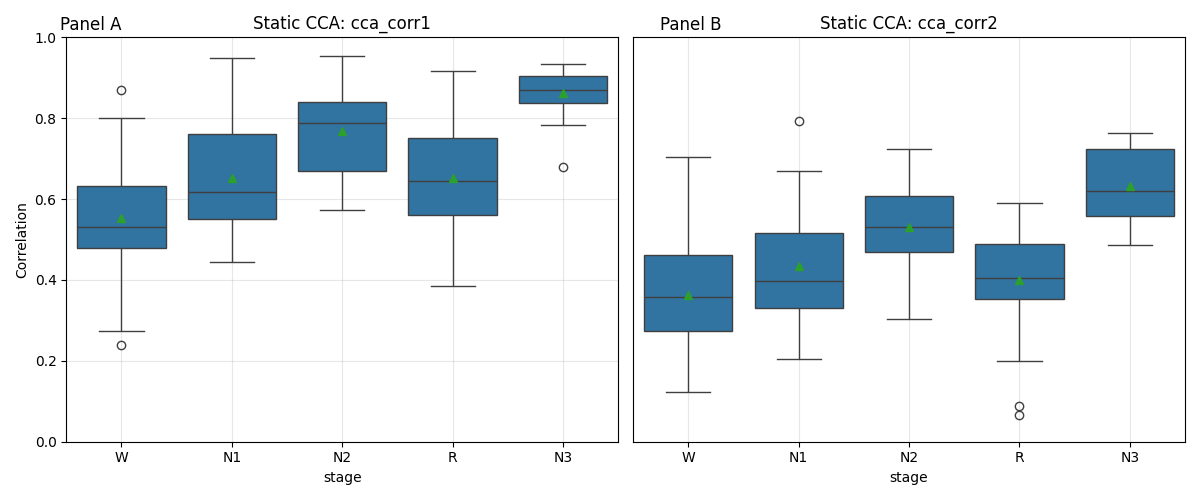
\includegraphics[width=0.8\textwidth]{figure1_static_cca_boxplots.png} % static_cca_analysis/cca_corr_by_stage.png
\caption{Static canonical correlation analysis (CCA) across sleep stages. Panel A shows the first canonical correlation ($\rho_1$), and Panel B shows the second ($\rho_2$), both increasing from Wake to N3.}\label{fig:figure1}
\end{figure}

\subsection{Time-Resolved CCA Analysis}

Sliding windows (30 s, $50\%$ overlap) reproduced the pattern with finer resolution. Aggregated $\rho_1$ ranged from 0.73 $\pm$ 0.13 (Wake) to 0.87 ± 0.07 (N3); $\rho_2$ from 0.45 $\pm$ 0.17 to 0.65 $\pm$ 0.11 (\ref{fig:figure2}). Variability diminished with depth, and 10-min bins revealed stable plateaus in N2/N3 but fluctuating profiles in REM and Wake. Transition phases (e.g., N1) showed inconsistent coupling patterns.

\begin{figure}
\centering
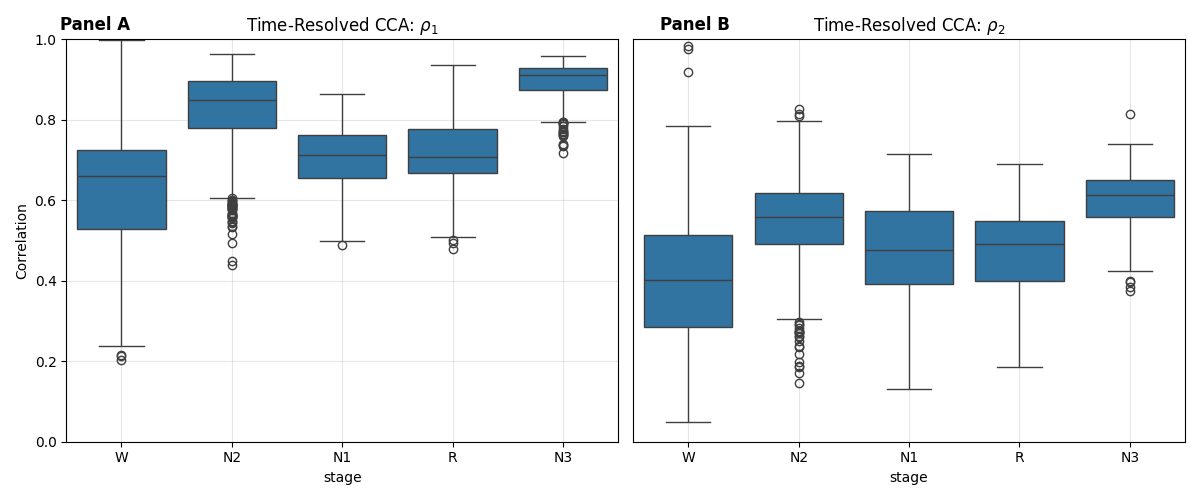
\includegraphics[width=0.8\textwidth]{figure2_time_resolved_boxplots.png} % static_cca_analysis/cca_corr_by_stage.png
\caption{Time-resolved CCA reveals stronger and more stable EEG-EOG coupling in deeper sleep stages.}\label{fig:figure2}
\end{figure}

\subsection{Distributional Complexity of Coupling Dynamics}

Entropy was highest in Wake and REM and lowest in N3 (\ref{fig:figure3}). Skewness (between -0.5 and 0.5) remained near zero, but kurtosis was elevated in Wake/REM, suggesting occasional extreme coupling events.

\begin{figure}
\centering
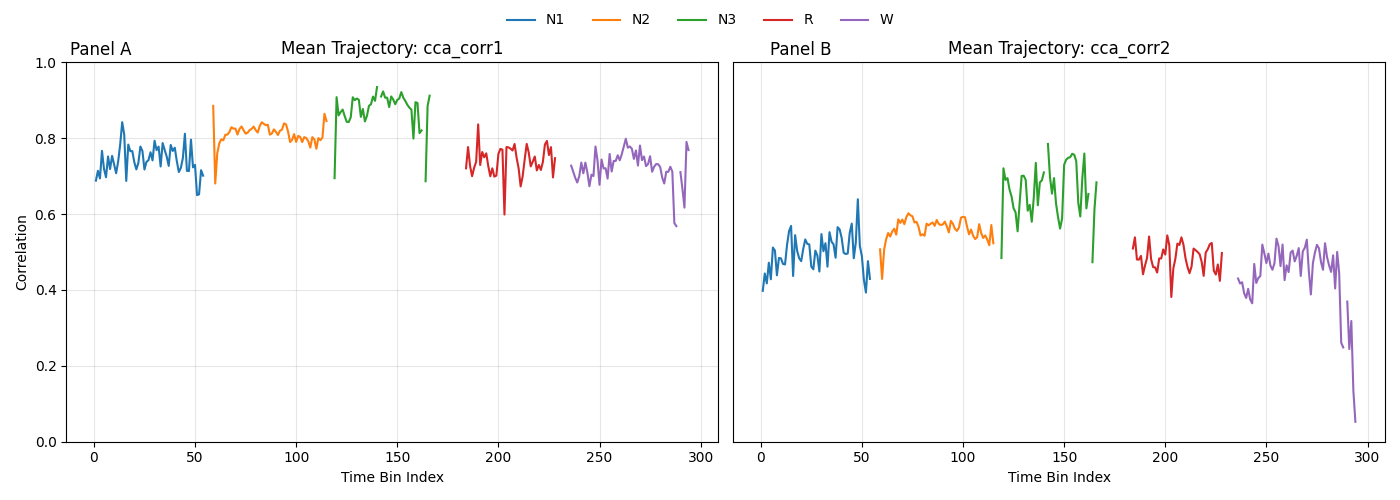
\includegraphics[width=0.8\textwidth]{figure3_cca_trajectories.png} % static_cca_analysis/cca_corr_by_stage.png
\caption{Coupling entropy is highest in Wake and REM, and lowest in N3.}\label{fig:figure3}
\end{figure}

\subsection{Projection Statistics and Downsampled Components}

Mean and variance of the individual canonical projections showed no stage effect (all ANOVA p > 0.17; \ref{fig:figure4}). Thus, stage differences stem from correlation structure rather than projection amplitude.

\begin{figure}
\centering
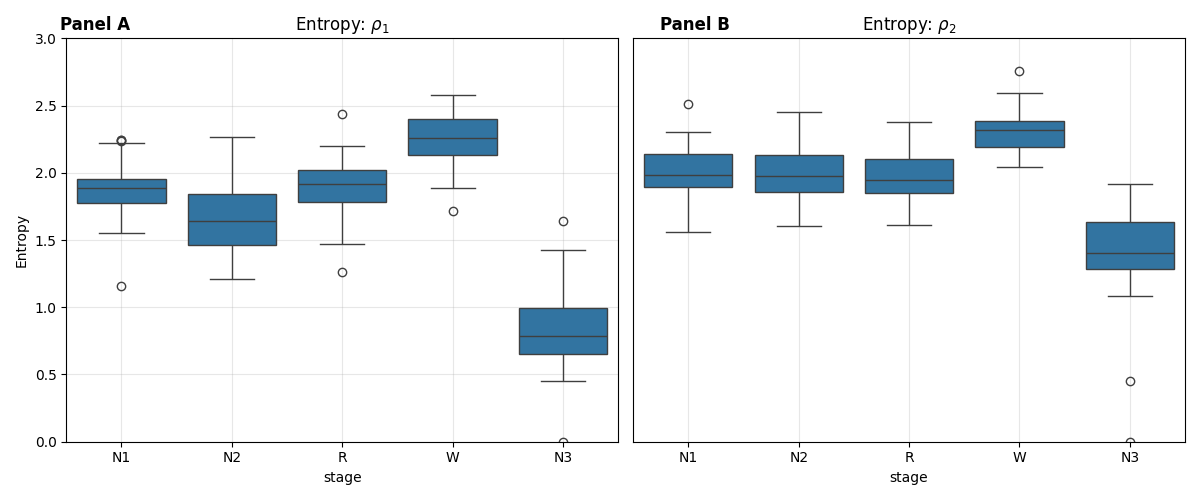
\includegraphics[width=0.8\textwidth]{figure4_entropy_boxplots.png}
\caption{Mean canonical projections remain stable across stages.}\label{fig:figure4}
\end{figure}

\section{Discussion}

This study quantified the low-dimensional communication subspace shared between EEG and EOG signals across sleep stages using CCA. Both static and time-resolved analyses revealed a robust increase in coupling strength with sleep depth: the first canonical correlation $\rho_1$ rose from 0.55$\pm$0.14 in Wake to 0.86$\pm$0.06 in N3, and the second $\rho_2$ from 0.36$\pm$0.15 to 0.63$\pm$0.10. REM and N1 showed intermediate coupling, closer to Wake than to N2/N3 --- a pattern replicated across time windows, further supporting the sleep-stage specificity of EEG-EOG coupling.
Temporal trajectories showed stable coupling in N2/N3 and greater variability in Wake and REM as they showing lower correlation values and higher entropy, supported by entropy measures. Lower entropy in deep sleep suggests more consistent EEG-EOG coordination, potentially reflecting reduced sensory input and motor variability. In contrast, higher entropy in Wake and REM may reflect more complex and dynamic brain-eye interactions. The persistent contribution of $\rho_2$ across all stages, especially in Wake and REM, suggests that EEG-EOG interactions are not dominated by a single mode, but instead reflect multiplexed coupling mechanisms in more active states.

\textbf{Limitations}
This study has several limitations. First, although preprocessing was applied, residual artifacts (e.g., blinks, muscle activity) may have influenced coupling estimates, especially in wake and REM stages. Second, the APPLES dataset includes individuals with varying sleep pathologies (e.g., OSAS), but we did not stratify by clinical status due to metadata constraints, limiting generalizability. Third, our analysis focused on a subset of EEG (C3, C4) and EOG (LOC, ROC) channels; while representative, this may miss spatially distributed coupling patterns. Fourth, our use of 10-minute time bins improved stability but may have smoothed out transient events during REM or stage transitions. Finally, CCA captures only linear relationships; incorporating nonlinear approaches (e.g., kernel CCA or mutual information) may reveal richer coupling dynamics in future work.

\section{Conclusion}
This study shows that EEG and EOG signals share a low-dimensional subspace whose strength and temporal stability vary systematically across sleep stages. Coupling was strongest and most consistent in N2 and N3, and more variable in Wake and REM. These findings suggest structured coordination between cortical and oculomotor systems that tracks sleep depth. By focusing on intermodality dynamics via CCA, our approach offers a compact, interpretable view of sleep architecture that may inform future studies of sleep disorders and altered states.

\renewcommand{\baselinestretch}{1.5}
%\singlespacing
%\renewcommand\bibname{Bibliography}
\bibliographystyle{abbrv} %abbrv
\phantomsection     % 
\cleardoublepage    % 
\bibliography{report}

\end{document}
